\documentclass{../../slides-style}

\slidetitle{Лекция 4: Архитектурные стили}{02.04.2024}

\begin{document}
    
    \begin{frame}[plain]
        \titlepage
    \end{frame}

    \section{Введение}

    \begin{frame}
        \frametitle{Архитектурные шаблоны и стили}
        Архитектурный стиль --- набор решений, которые
        \begin{enumerate}
            \item применимы в выбранном контексте разработки,
            \item задают ограничения на принимаемые архитектурные решения, специфичные для определённых систем в этом контексте,
            \item приводят к желаемым положительным качествам получаемой системы.
        \end{enumerate}
        Архитектурный шаблон --- именованный набор ключевых проектных решений по эффективной организации подсистем, применимых для повторяемых технических задач проектирования в различных контекстах и предметных областях
    \end{frame}

    \begin{frame}
        \frametitle{Архитектурные шаблоны и стили, классификация}
        \begin{center}
            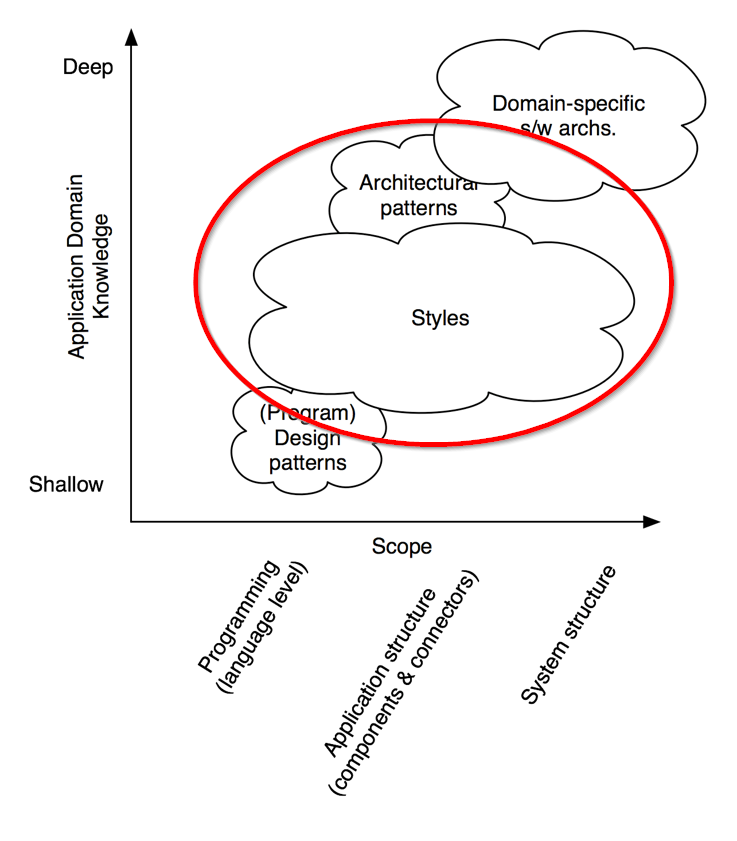
\includegraphics[width=0.5\textwidth]{architecturalStylesHighlighted.png}
            \attribution{N. Medvidovic}
        \end{center}
    \end{frame}

    \section{Примеры архитектурных шаблонов}

    \begin{frame}
        \frametitle{Пример: трёхзвенная архитектура}
        \framesubtitle{State-Logic-Display}
        \begin{columns}
            \begin{column}{0.5\textwidth}
                Примеры применения
                \begin{itemize}
                    \item Бизнес-приложения
                    \item Многопользовательские игры
                    \item Веб-приложения
                \end{itemize}
            \end{column}
            \begin{column}{0.5\textwidth}
                \begin{center}
                    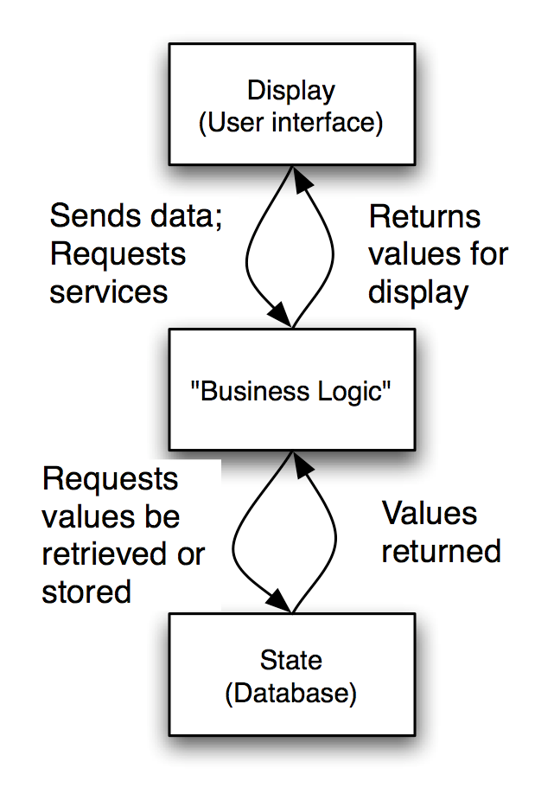
\includegraphics[width=0.7\textwidth]{threeTieredArchitecture.png}
                    \attribution{N. Medvidovic}
                \end{center}
            \end{column}
        \end{columns}
    \end{frame}

    \begin{frame}
        \frametitle{Пример: Model-View-Controller}
        \begin{center}
            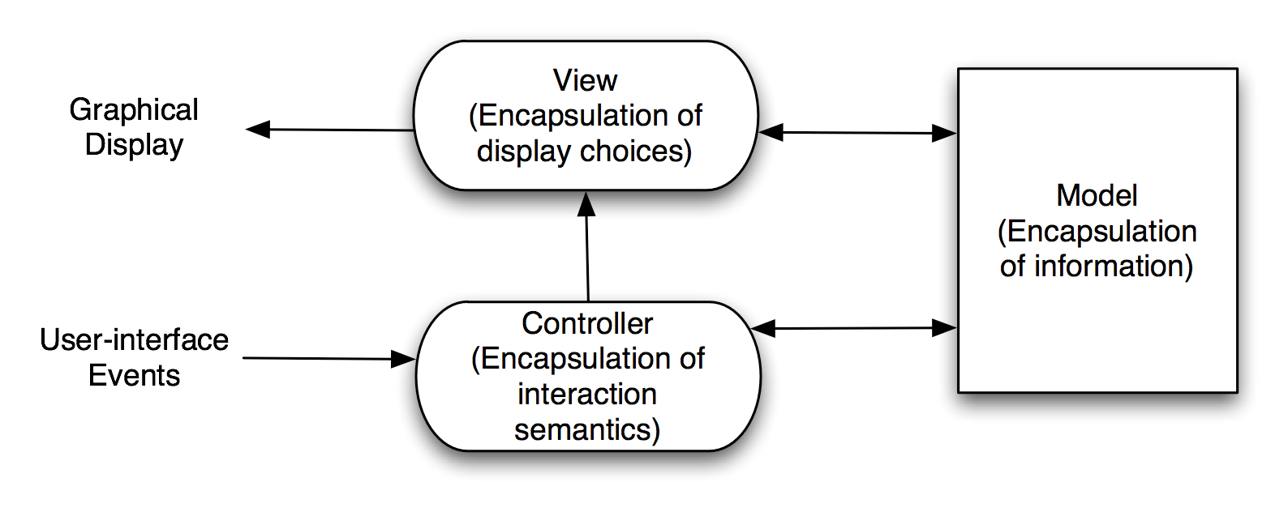
\includegraphics[width=0.65\textwidth]{mvc.png}
            \attribution{N. Medvidovic}
        \end{center}
        \begin{itemize}
            \item Разделяет данные, представление и взаимодействие с пользователем
            \item Если в модели что-то меняется, она оповещает представление (представления)
            \item Через контроллер проходит всё взаимодействие с пользователем
            \begin{itemize}
                \item Естественное место для паттерна ``Команда'' и Undo/Redo
            \end{itemize}
        \end{itemize}
    \end{frame}

    \begin{frame}
        \frametitle{Пример: Sense-Compute-Control}
        \begin{center}
            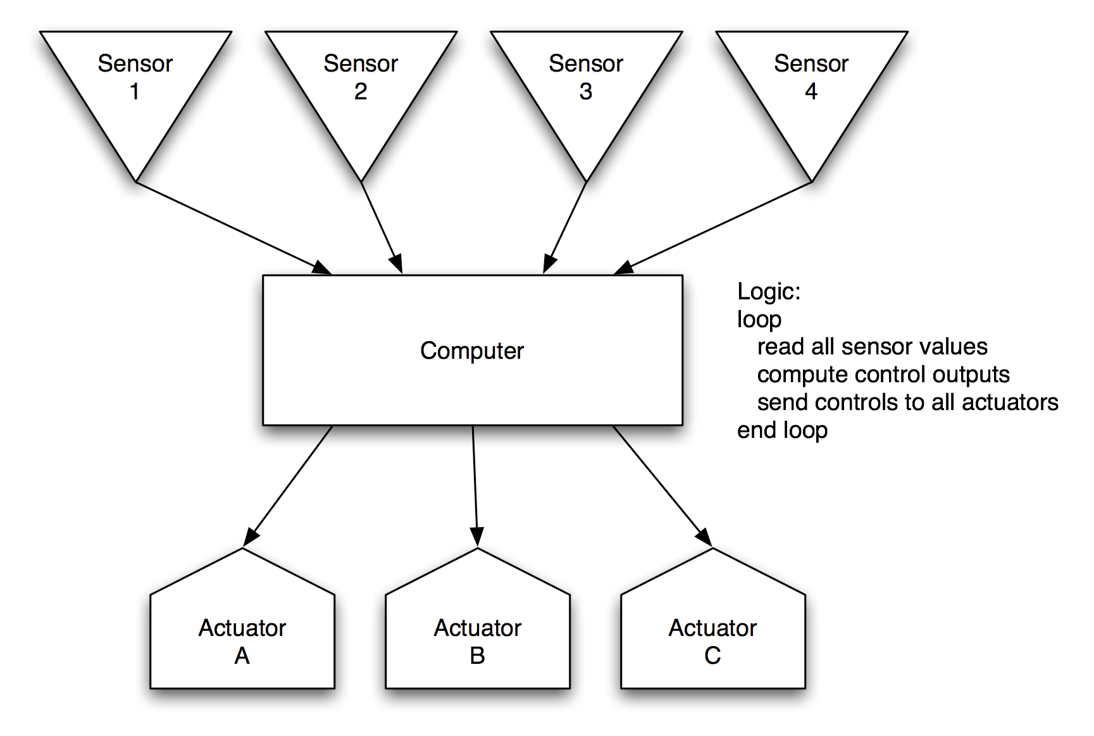
\includegraphics[width=0.65\textwidth]{senseComputeControl.png}
            \attribution{N. Medvidovic}
        \end{center}
        \begin{itemize}
            \item Применяется во встроенных системах и робототехнике
        \end{itemize}
    \end{frame}

    \section{Архитектурные стили}

    \begin{frame}
        \frametitle{Архитектурные стили}
        \begin{itemize}
            \item Именованная коллекция архитектурных решений
            \item Менее узкоспециализированные, чем архитектурные паттерны
        \end{itemize}
        \begin{center}
            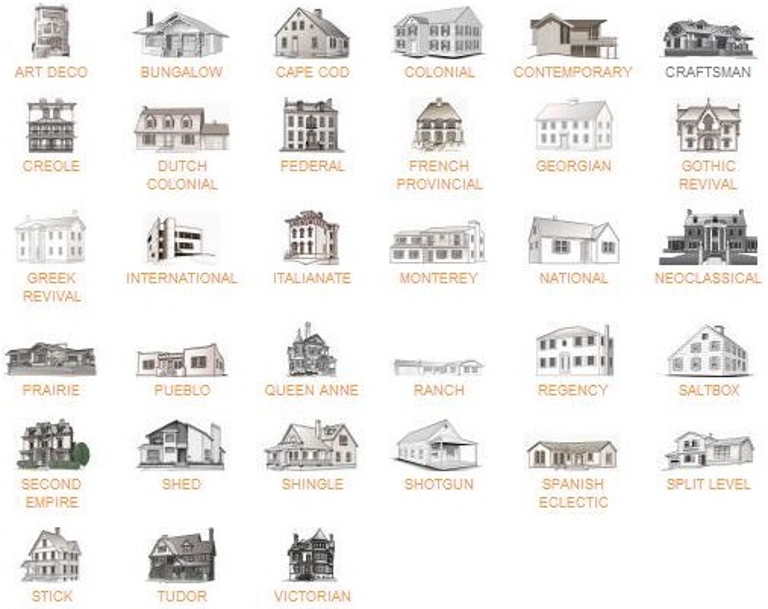
\includegraphics[width=0.5\textwidth]{buildingStyles.png}
            \attribution{N. Medvidovic}
        \end{center}
    \end{frame}

    \begin{frame}
        \frametitle{Архитектурные стили}
        \begin{columns}
            \begin{column}{0.5\textwidth}
                \begin{itemize}
                    \item Одна система может включать в себя несколько архитектурных стилей
                    \item Понятие стиля применимо и к подсистемам
                \end{itemize}
            \end{column}
            \begin{column}{0.5\textwidth}
                \begin{center}
                    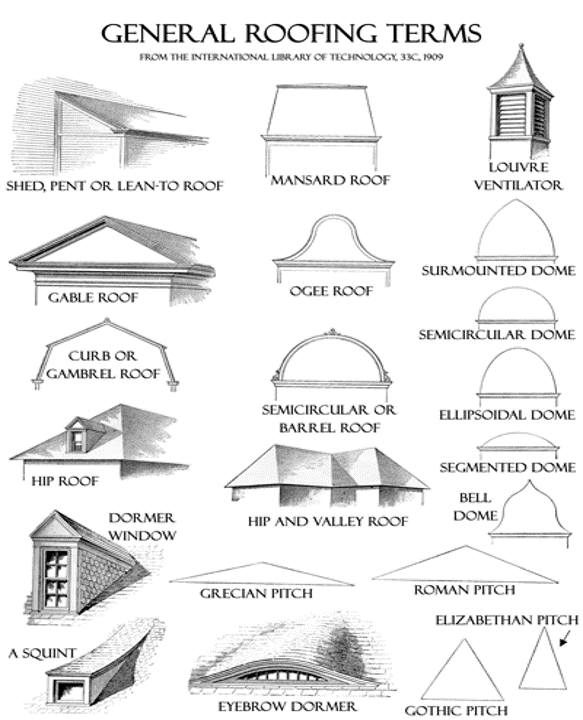
\includegraphics[width=0.7\textwidth]{roofStyles.png}
                    \attribution{N. Medvidovic}
                \end{center}
            \end{column}
        \end{columns}
    \end{frame}

    \begin{frame}
        \frametitle{Преимущества использования стилей}
        \begin{itemize}
            \item Переиспользование архитектуры
            \begin{itemize}
                \item Для новых задач можно применять хорошо известные и изученные решения
            \end{itemize}
            \item Переиспользование кода
            \begin{itemize}
                \item Часто у стилей бывают неизменяемые части, которые можно один раз реализовать
            \end{itemize}
            \item Упрощение общения и понимания системы
            \item Упрощение интеграции приложений
            \item Специфичные для стиля методы анализа
            \begin{itemize}
                \item Возможны благодаря ограничениям на структуру системы
            \end{itemize}
            \item Специфичные для стиля методы визуализации
        \end{itemize}
    \end{frame}

    \begin{frame}
        \frametitle{Основные характеристики стилей}
        \begin{itemize}
            \item Набор используемых элементов архитектуры
            \begin{itemize}
                \item Типы компонентов и соединителей, элементы данных
                \begin{itemize}
                    \item Например, объекты, фильтры, сервера и т.д.
                \end{itemize}
            \end{itemize}
            \item Набор правил конфигурирования
            \begin{itemize}
                \item ``Топологические'' ограничения на соединение элементов
                \begin{itemize}
                    \item Например, компонент может быть соединён с максимум двумя компонентами
                \end{itemize}
            \end{itemize}
            \item Семантика, стоящая за элементами
        \end{itemize}
    \end{frame}

    \section{Объектно-ориентированный стиль}

    \begin{frame}
        \frametitle{``Сырой'' объектно-ориентированный стиль}
        \begin{itemize}
            \item Компоненты --- объекты
            \item Соединители --- сообщения и вызовы методов
            \item Инварианты:
            \begin{itemize}
                \item Объекты отвечают за своё внутреннее состояние
                \item Реализация скрыта от других объектов
            \end{itemize}
            \item Преимущества:
            \begin{itemize}
                \item Декомпозиция системы в набор взаимодействующих агентов
                \item Внутреннее представление объектов можно менять независимо
                \item Близко к предметной области
            \end{itemize}
            \item Недостатки:
            \begin{itemize}
                \item Побочные эффекты при вызове методов
                \item Объекты вынуждены знать обо всех, от кого зависят
            \end{itemize}
        \end{itemize}
    \end{frame}

    \section{Слоистый стиль}

    \begin{frame}
        \frametitle{Слоистый стиль}
        \framesubtitle{Layered style}
        \begin{itemize}
            \item Иерархическая организация системы
            \begin{itemize}
                \item ``Многоуровневый клиент-сервер''
                \item Каждый слой предоставляет интерфейс для использования слоями выше
            \end{itemize}
            \item Каждый слой работает как:
            \begin{itemize}
                \item Сервер --- предоставляет функциональность слоям выше
                \item Клиент --- использует функциональность слоёв ниже
            \end{itemize}
            \item Соединители --- протоколы взаимодействия слоёв
            \item Пример --- операционные системы, сетевые стеки протоколов
        \end{itemize}
    \end{frame}

    \begin{frame}
        \frametitle{Слоистый стиль, подробности}
        \begin{columns}
            \begin{column}{0.5\textwidth}
                \begin{itemize}
                    \item Преимущества:
                    \begin{itemize}
                        \item Повышение уровня абстракции
                        \item Лёгкость в расширении
                        \item Изменения в каждом уровне затрагивают максимум два соседних
                        \item Возможны разные реализации уровня, если они удовлетворяют интерфейсу
                    \end{itemize}
                    \item Недостатки:
                    \begin{itemize}
                        \item Не всегда применим
                        \item Проблемы с производительностью
                    \end{itemize}
                \end{itemize}
            \end{column}
            \begin{column}{0.5\textwidth}
                \begin{center}
                    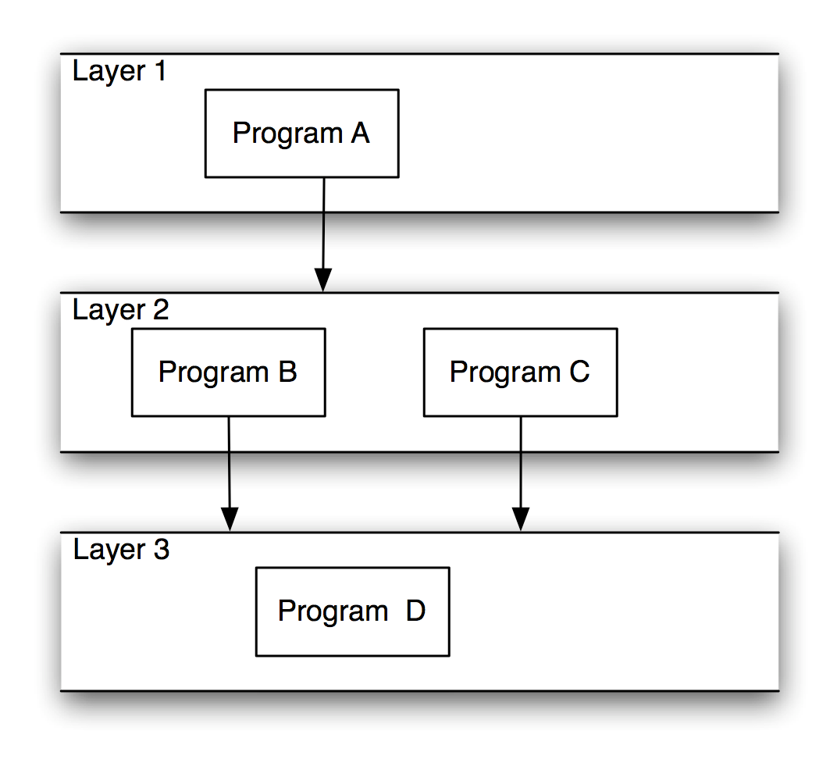
\includegraphics[width=0.8\textwidth]{layered.png}
                    \attribution{N. Medvidovic}
                \end{center}
            \end{column}
        \end{columns}
    \end{frame}

    \begin{frame}
        \frametitle{Пример}
        \framesubtitle{Стандартные слои в Domain-Driven Design}
        \begin{center}
            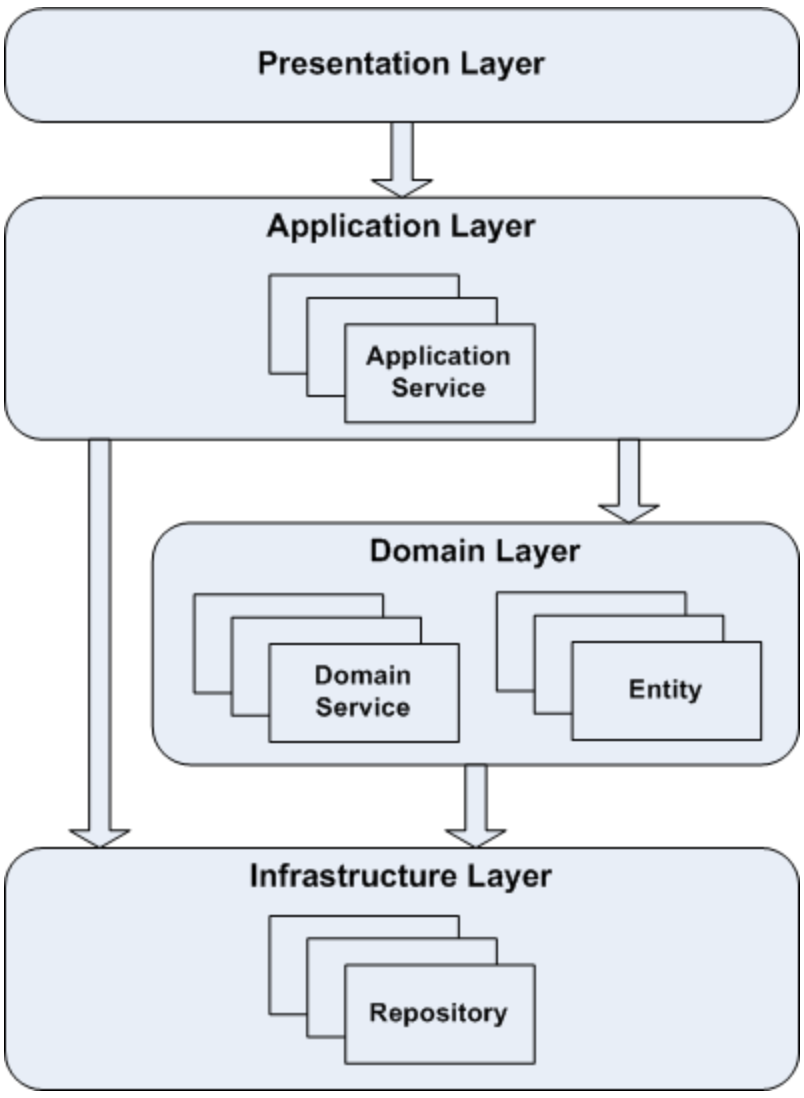
\includegraphics[width=0.35\textwidth]{dddLayers.png}
            \begin{scriptsize}
                \attribution{\url{http://uniknow.github.io/AgileDev/site/0.1.8-SNAPSHOT/parent/ddd/core/layered_architecture.html}}
            \end{scriptsize}
        \end{center}
    \end{frame}

    \section{Клиент-сервер}

    \begin{frame}
        \frametitle{``Клиент-сервер''}
        \begin{itemize}
            \item Компоненты --- клиенты и серверы
            \item Серверы не знают ничего о клиентах, даже их количество
            \item Клиенты знают только про сервера и не могут общаться друг с другом
            \item Соединители --- сетевые протоколы
        \end{itemize}
    \end{frame}

    \section{Гексагональная архитектура}

    \begin{frame}
        \frametitle{Гексагональная архитектура}
        \framesubtitle{``Порты и адаптеры''}
        \begin{columns}
            \begin{column}{0.5\textwidth}
                \begin{itemize}
                    \item Другая точка зрения на уровни: самый нижний --- уровень предметной области
                    \item Всё остальное поставляется ему как внешние зависимости
                    \item Активно используется Dependency Inversion
                    \item Порт --- по сути, интерфейс, предоставляемый или потребляемый
                    \item Адаптер --- паттерн ``Адаптер'' для ``подгонки'' интерфейсов
                \end{itemize}
            \end{column}
            \begin{column}{0.5\textwidth}
                \begin{center}
                    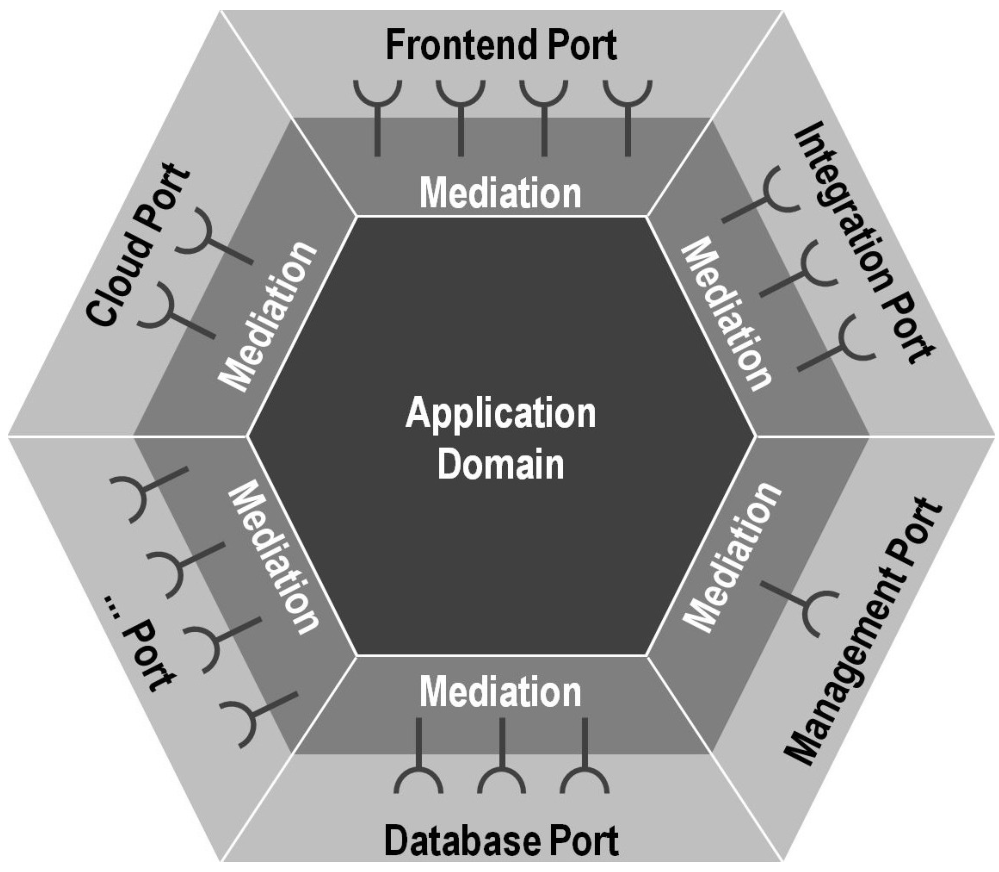
\includegraphics[width=0.8\textwidth]{hexagonalArchitecture.png}
                    \attribution{B Butzin et al, Microservices Approach for the Internet of Things}
                \end{center}
            \end{column}
        \end{columns}
    \end{frame}

    \begin{frame}
        \frametitle{Подробности}
        \begin{center}
            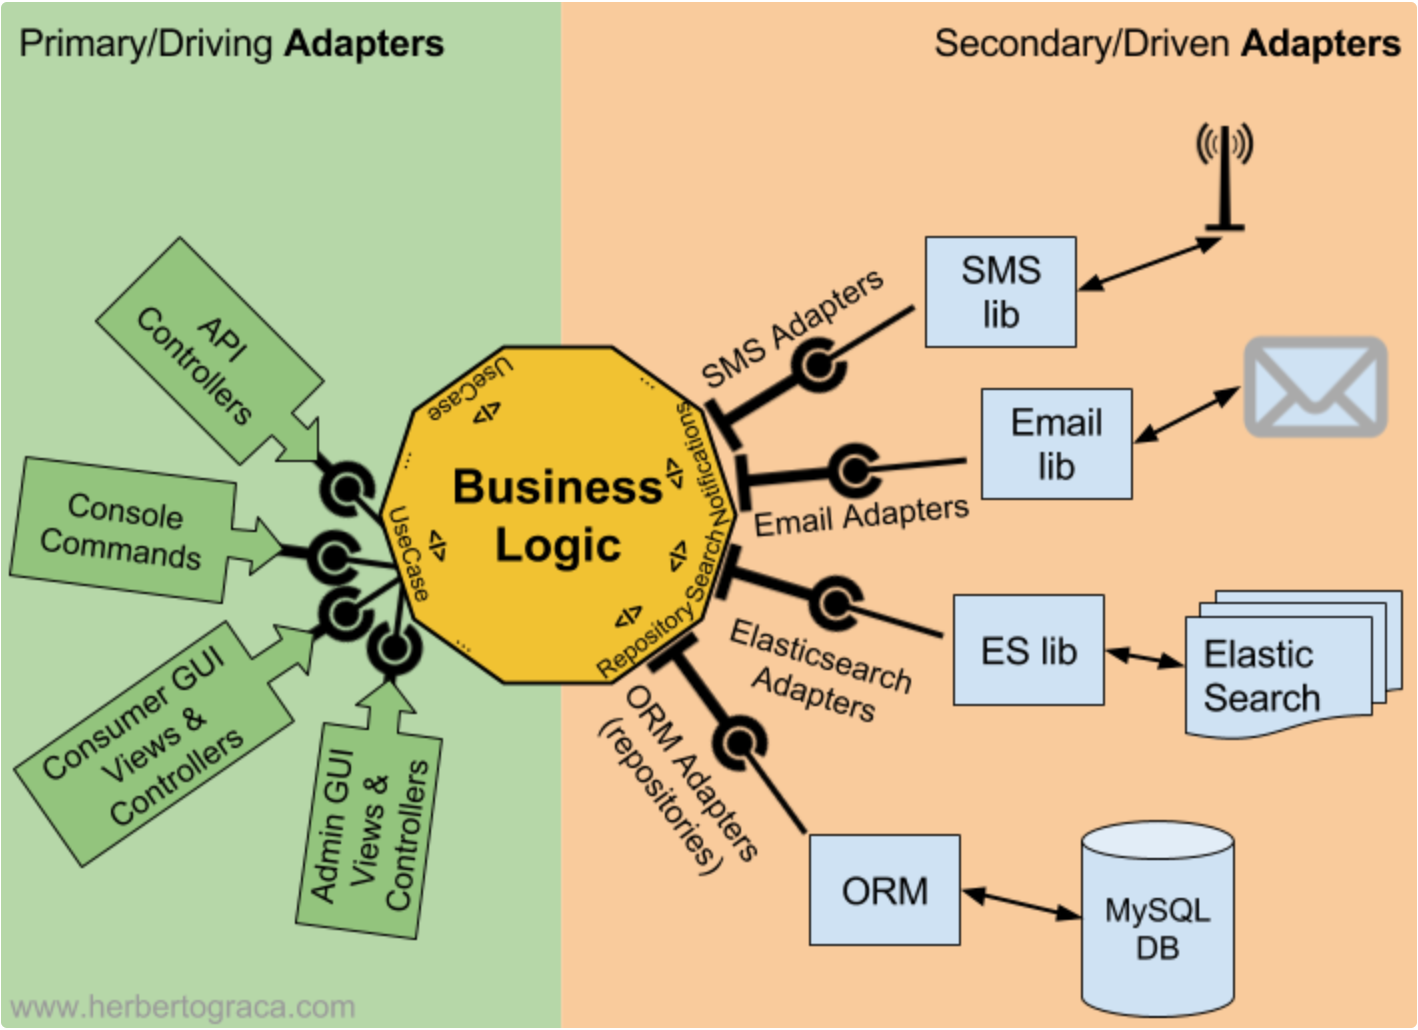
\includegraphics[width=0.8\textwidth]{hexagonalArchitectureDetails.png}
            \attribution{\url{https://herbertograca.com/2017/09/14/ports-adapters-architecture/}}
        \end{center}
    \end{frame}

    \begin{frame}
        \frametitle{Плюсы и минусы}
        Плюсы:
        \begin{itemize}
            \item Изоляция механизмов доставки
            \item Изоляция вспомогательных механизмов
            \item Лёгкость тестирования, моки
            \item Чистая бизнес-логика и модель предметной области
            \begin{itemize}
                \item Максимальная простота
                \item Возможность валидации и конвертирования данных
            \end{itemize}
        \end{itemize}
        \vspace{5mm}
        Минусы:
        \begin{itemize}
            \item Довольно тяжеловесна
            \item Непонятно, что делать с фреймворками
            \item Не очень подробна
        \end{itemize}
    \end{frame}

    \section{Луковая архитектура}

    \begin{frame}
        \frametitle{Луковая архитектура}
        \begin{columns}
            \begin{column}{0.5\textwidth}
                \begin{itemize}
                    \item Дальнейшее развитие гексагональной --- определяет внутреннюю структуру ядра
                    \item Внутренние слои не знают о внешних, доменная модель вообще ни о ком не знает
                    \item Внутренние слои определяют интерфейсы, внешние их реализуют
                    \item Уровневость нестрогая --- слой может использовать все слои под ним
                \end{itemize}
            \end{column}
            \begin{column}{0.5\textwidth}
                \begin{center}
                    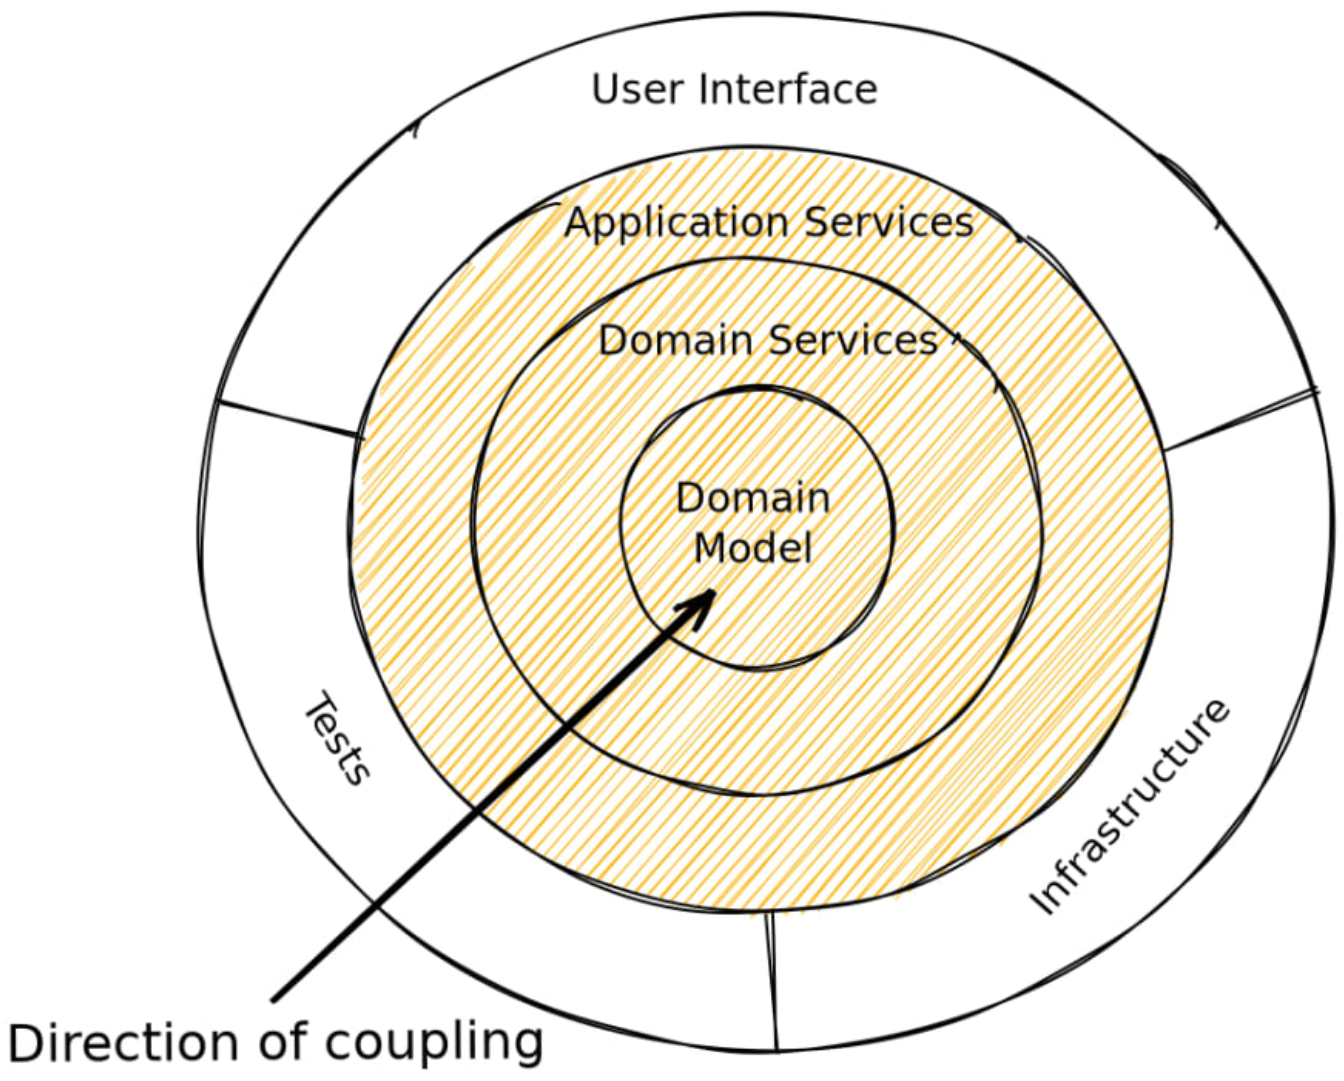
\includegraphics[width=0.8\textwidth]{onionArchitecture.png}
                    \attribution{https://dev.to/barrymcauley/onion-architecture-3fgl}
                \end{center}
            \end{column}
        \end{columns}
    \end{frame}

    \begin{frame}
        \frametitle{Подробности}
        \begin{center}
            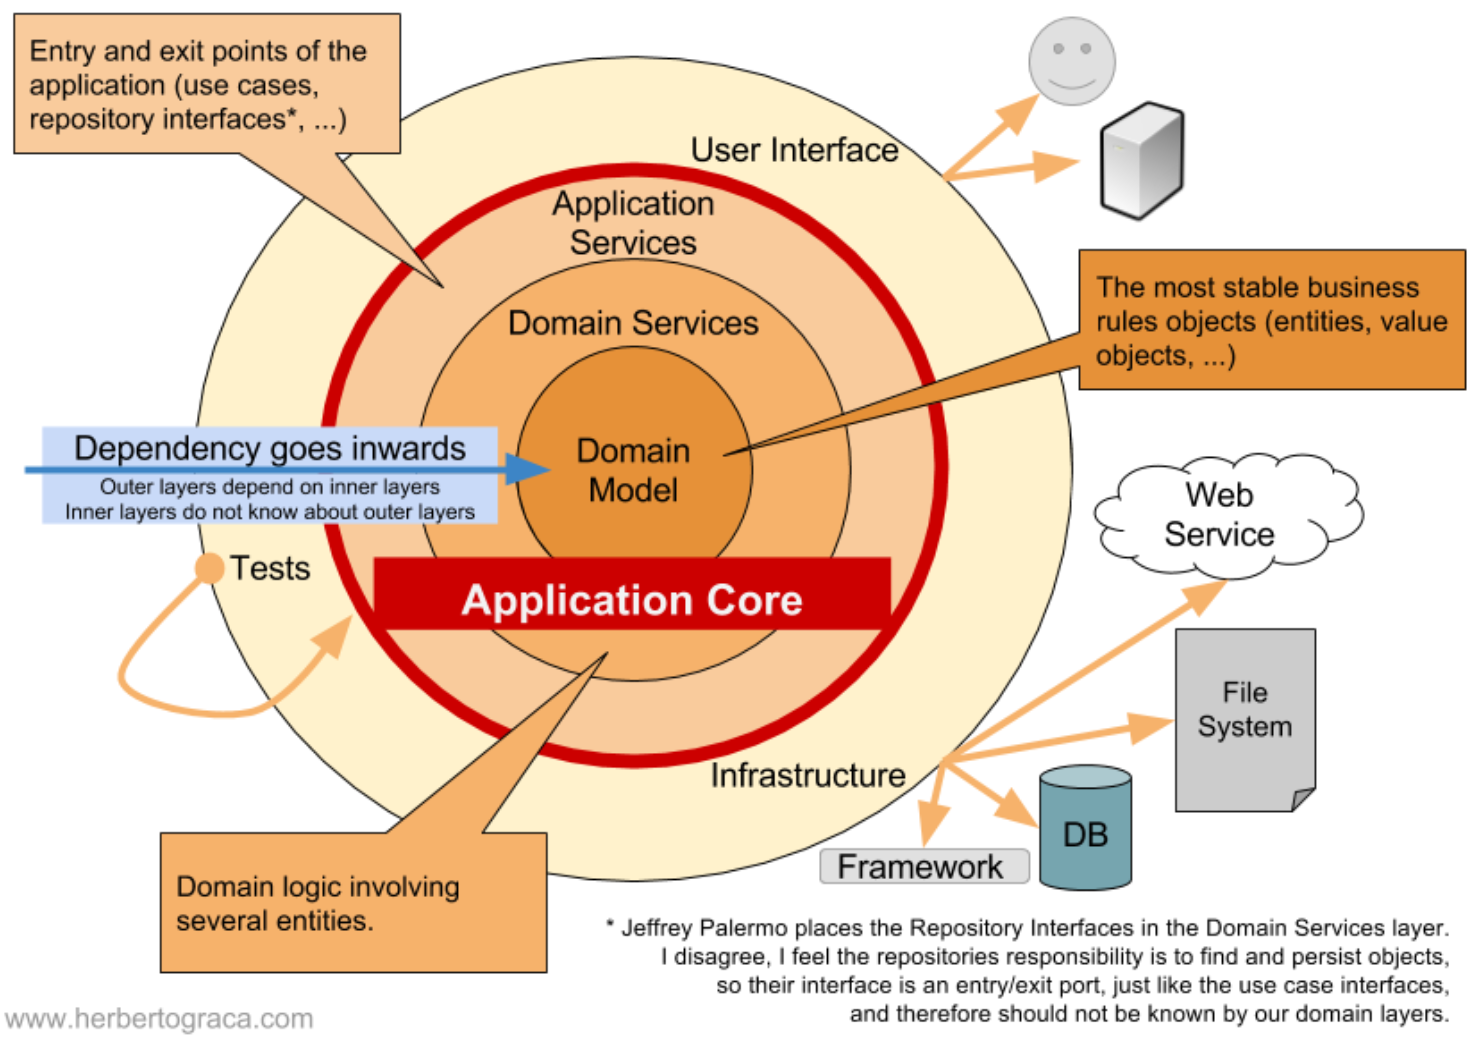
\includegraphics[width=0.75\textwidth]{onionArchitectureDetails.png}
            \attribution{\url{https://herbertograca.com/2017/09/21/onion-architecture/}}
        \end{center}
    \end{frame}

    \section{Чистая архитектура}

    \begin{frame}
        \frametitle{Чистая архитектура}
        \begin{center}
            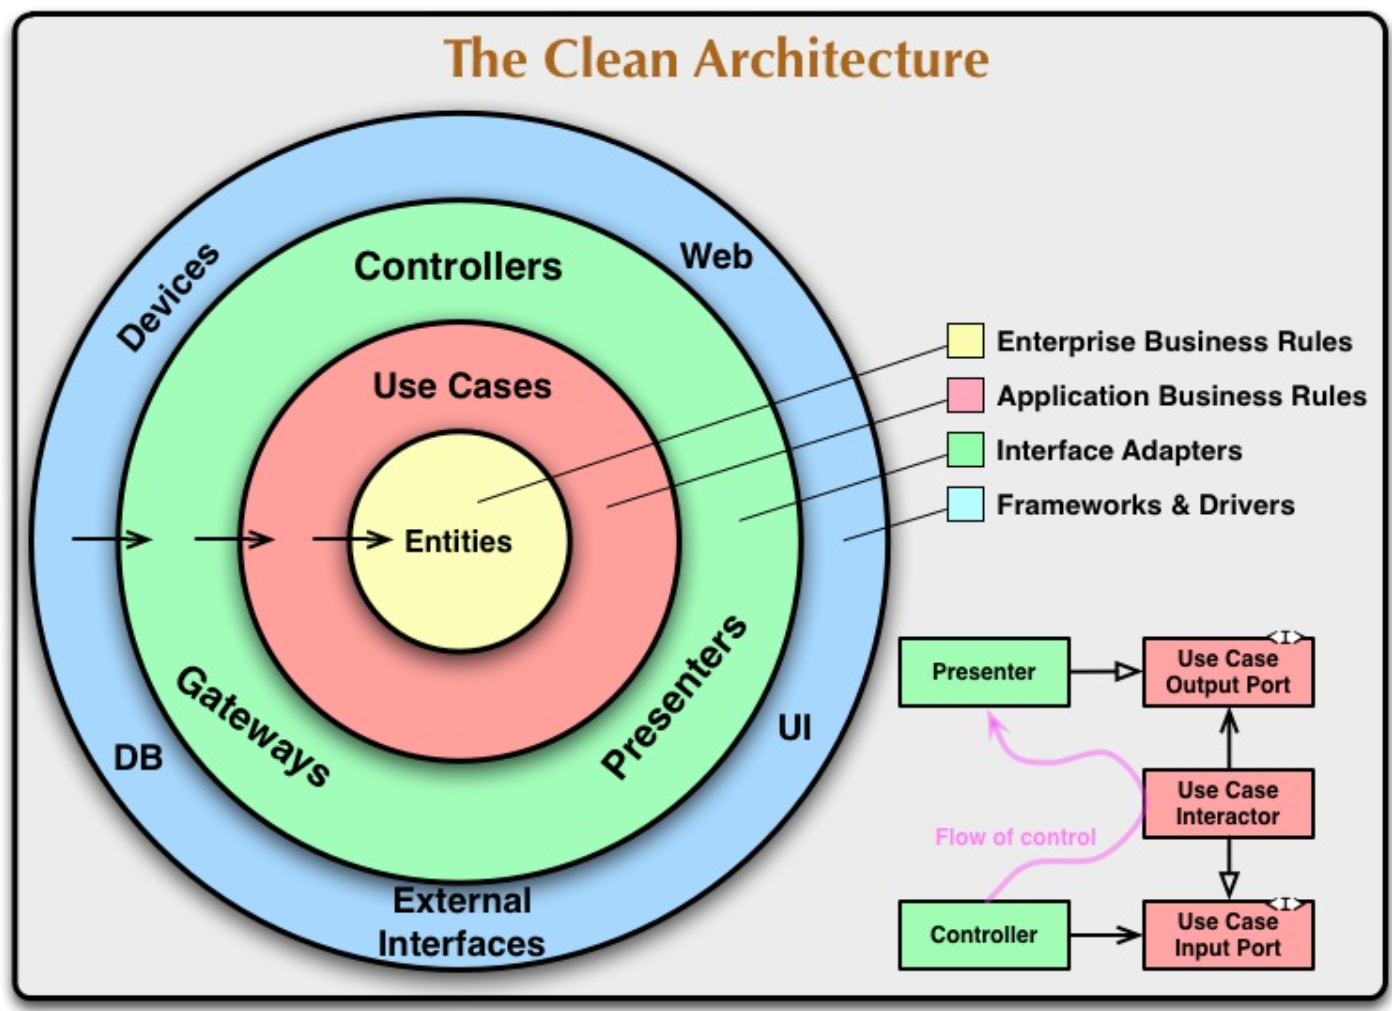
\includegraphics[width=0.6\textwidth]{cleanArchitecture.png}
            \attribution{https://herbertograca.com/2017/09/28/clean-architecture-standing-on-the-shoulders-of-giants/}
        \end{center}
        \begin{itemize}
            \item Дальнейшее развитие луковой --- определяет поток управления
        \end{itemize}
    \end{frame}

    \begin{frame}
        \frametitle{Чистая архитектура, обработка запроса}
        \begin{center}
            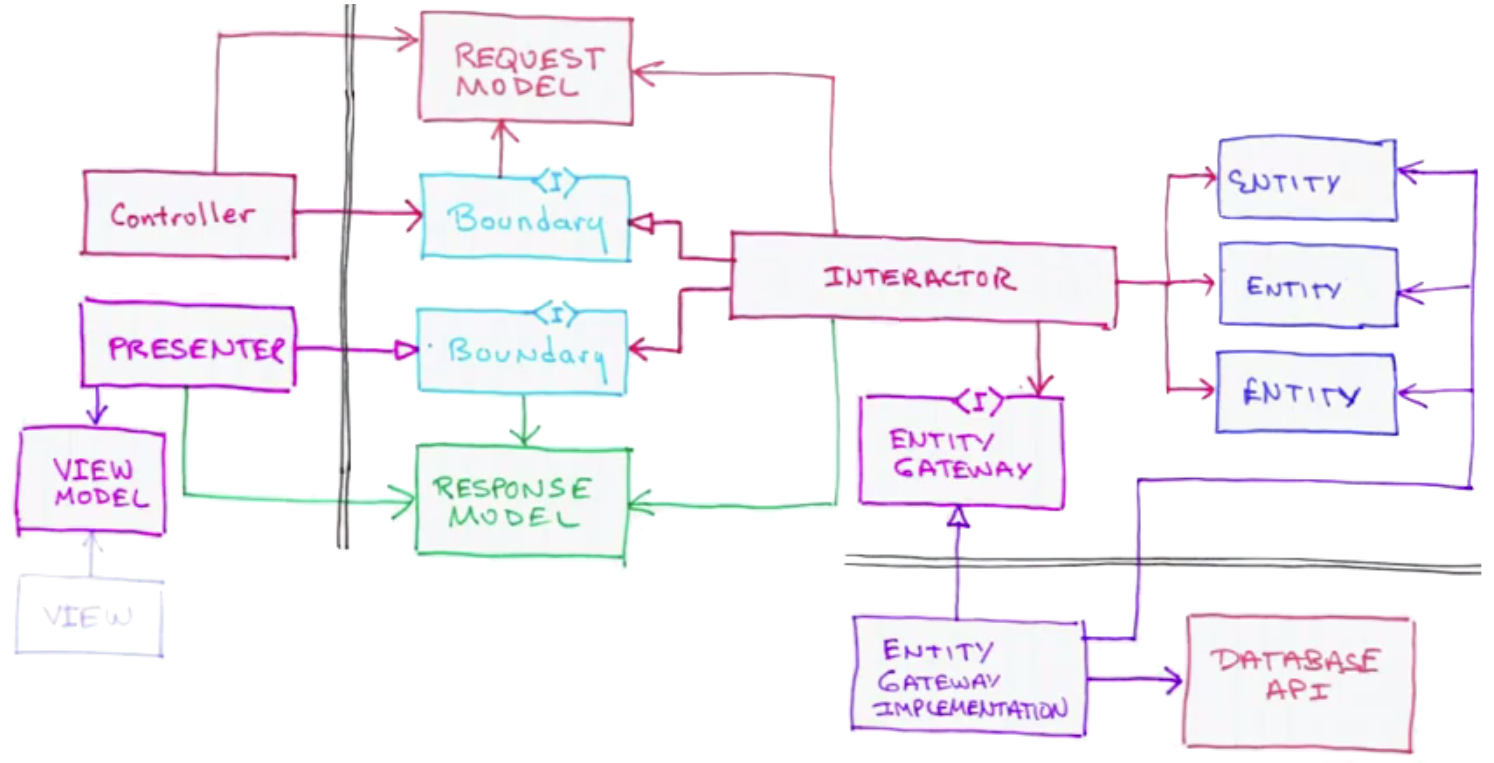
\includegraphics[width=0.8\textwidth]{cleanArchitectureControlFlow.png}
            \attribution{https://herbertograca.com/2017/09/28/clean-architecture-standing-on-the-shoulders-of-giants/}
        \end{center}
    \end{frame}

    \section{Пакетная обработка}

    \begin{frame}
        \frametitle{Пакетная обработка}
        \begin{itemize}
            \item Система строится как набор отдельных программ, выполняющихся последовательно
            \item Данные стандартным для ОС способом передаются от программы к программе
            \begin{itemize}
                \item Pipes, named pipes, файлы
            \end{itemize}
            \item Данные --- в явном виде всё, необходимое для работы
        \end{itemize}
        Типичен для финансовых систем глубокой древности (``Прадедушка стилей'')
        \begin{center}
            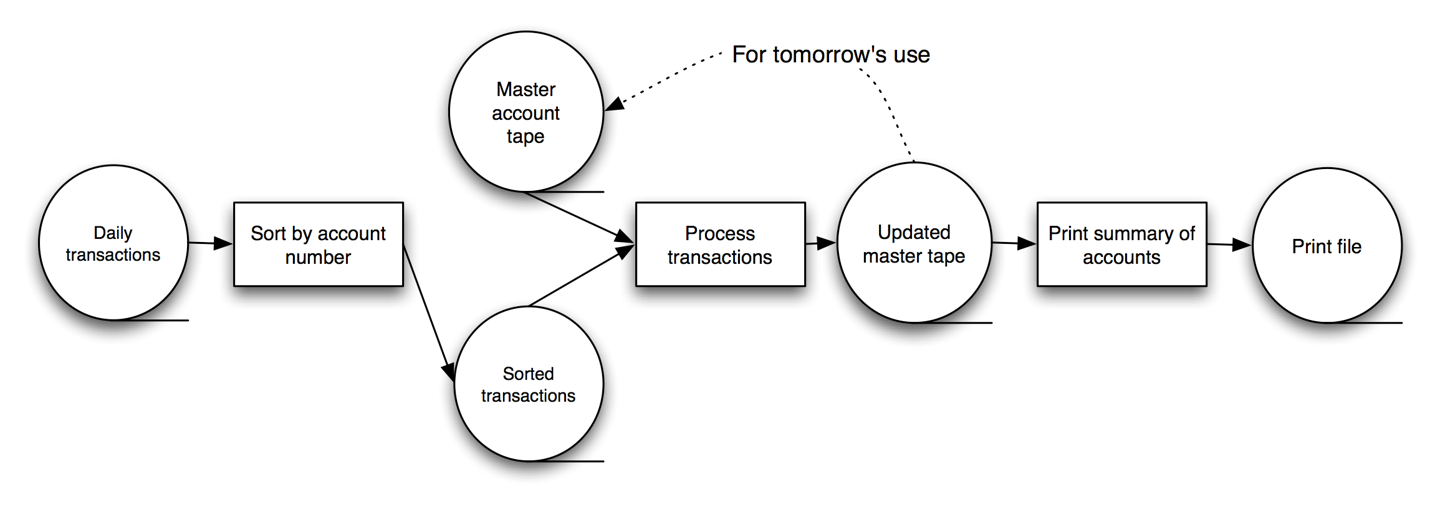
\includegraphics[width=0.7\textwidth]{batch.png}
            \attribution{N. Medvidovic}
        \end{center}
    \end{frame}

    \section{Каналы и фильтры}

    \begin{frame}
        \frametitle{Каналы и фильтры}
        \framesubtitle{Pipes and filters}
        \begin{itemize}
            \item Компоненты --- это фильтры, преобразующие данные из входных каналов в данные в выходных каналах
            \item Соединители --- каналы
            \item Инварианты:
            \begin{itemize}
                \item Фильтры независимы (не имеют разделяемого состояния)
                \item Фильтры не знают о фильтрах до или после них
            \end{itemize}
            \item Вариации:
            \begin{itemize}
                \item Конвейеры --- линейные последовательности фильтров
                \item Ограниченные каналы --- где канал это очередь с ограниченным количеством элементов
                \item Типизированные каналы --- где каналы отличаются по типу передаваемых данных
            \end{itemize}
        \end{itemize}
    \end{frame}

    \begin{frame}
        \frametitle{Каналы и фильтры, подробности}
        \begin{itemize}
            \item Преимущества:
            \begin{itemize}
                \item Поведение системы --- это просто последовательное применение поведений компонентов
                \item Легко добавлять, заменять и переиспользовать фильтры
                \begin{itemize}
                    \item Любые два фильтра можно использовать вместе
                \end{itemize}
                \item Широкие возможности для анализа
                \begin{itemize}
                    \item Пропускная способность, задержки, deadlock-и
                \end{itemize}
                \item Широкие возможности для параллелизма
            \end{itemize}
            \item Недостатки:
            \begin{itemize}
                \item Последовательное исполнение
                \item Проблемы с интерактивными приложениями
                \item Пропускная способность определяется самым ``узким'' элементом
            \end{itemize}
        \end{itemize}
    \end{frame}

    \section{Blackboard}

    \begin{frame}
        \frametitle{Blackboard}
        \begin{itemize}
            \item Два типа компонентов:
            \begin{itemize}
                \item Центральная структура данных --- та самая ``Blackboard''
                \item Компоненты, работающие с blackboard
            \end{itemize}
            \item Инварианты:
            \begin{itemize}
                \item Управление системой осуществляется только через состояние доски
                \item Компоненты не знают друг о друге и не имеют своего состояния
            \end{itemize}
            \item Системы переписывающих правил --- некоторые задачи ИИ, трансляторы, графовые грамматики, алгорифмы Маркова
        \end{itemize}
    \end{frame}

    \section{Событийный стиль}

    \begin{frame}
        \frametitle{Событийный стиль}
        \begin{itemize}
            \item Оповещение о событии вместо явного вызова метода
            \begin{itemize}
                \item ``Слушатели'' могут подписаться на событие
                \item Система при наступлении события сама вызывает все зарегистрированные методы слушателей
            \end{itemize}
            \item Компоненты имеют два вида интерфейсов --- методы и события
            \item Два типа соединителей:
            \begin{itemize}
                \item Явный вызов метода
                \item Неявный вызов по наступлению события
            \end{itemize}
            \item Инварианты:
            \begin{itemize}
                \item Те, кто производит события, не знают, кто и как на них отреагирует
                \item Не делается никаких предположений о том, как событие будет обработано и будет ли вообще
            \end{itemize}
        \end{itemize}
    \end{frame}

    \begin{frame}
        \frametitle{Событийный стиль, преимущества и недостатки}
        \begin{itemize}
            \item Преимущества:
            \begin{itemize}
                \item Переиспользование компонентов
                \begin{itemize}
                    \item Очень низкая связность между компонентами
                \end{itemize}
                \item Лёгкость в конфигурировании системы
                \begin{itemize}
                    \item Как во время компиляции, так и во время выполнения
                \end{itemize}
            \end{itemize}
            \item Недостатки:
            \begin{itemize}
                \item Зачастую неинтуитивная структура системы
                \item Компоненты не управляют последовательностью вычислений
                \item Непонятно, кто отреагирует на запрос и в каком порядке придут ответы
                \item Тяжело отлаживаться
                \item Гонки даже в однопоточном приложении
            \end{itemize}
        \end{itemize}
    \end{frame}

    \section{Publish-subscribe}

    \begin{frame}
        \frametitle{Издатель-подписчик}
        \framesubtitle{Publish-subscribe}
        \begin{itemize}
            \item Подписчики регистрируются, чтобы получать нужные им сообщения или данные. Издатели публикуют сообщения, синхронно или асинхронно.
            \item Компоненты: издатели, подписчики, ``маршрутизаторы''
            \item Соединители: как правило, сетевые протоколы, часто механизм наподобие паттерна ``Наблюдатель''
            \item Данные: подписки, нотификации, публикуемая информация
            \item Топология: подписчики подключаются к издателям напрямую, либо через посредников
            \item Преимущества: очень низкая связность между компонентами, при этом высокая эффективность распределения информации
        \end{itemize}
    \end{frame}

    \section{Событийная шина}

    \begin{frame}
        \frametitle{Событийная шина}
        \begin{itemize}
            \item Независимые компоненты посылают и принимают события, передаваемые по шинам
            \item Компоненты: независимые генераторы или потребители событий
            \item Соединители: шины событий (хотя бы одна)
            \item Данные: события и связанные с ними данные, посылаемые по шине
            \item Топология: компоненты общаются только с шинами событий, не друг с другом
            \item Варианты: push- и pull-режимы работы с шиной
            \item Преимущества: лёгкость масштабирования и добавления новой функциональности, эффективно для распределённых приложений
            \item Event Sourcing
        \end{itemize}
    \end{frame}

    \section{Peer-to-peer}

    \begin{frame}
        \frametitle{Peer-to-peer}
        \begin{itemize}
            \item Состояние и поведение распределены между компонентами, которые могут выступать как клиенты и как серверы
            \item Компоненты: имеют своё состояние и свой поток управления
            \item Соединители: как правило, сетевые протоколы
            \item Элементы данных: сетевые сообщения
            \item Топология: сеть (возможно, с избыточными связями между компонентами), может динамически меняться
            \item Преимущества:
            \begin{itemize}
                \item Хорош для распределённых вычислений
                \item Устойчив к отказам
                \item Если протокол взаимодействия позволяет, легко масштабируется
            \end{itemize}
        \end{itemize}
    \end{frame}

\end{document}